%% This is an example first chapter.  You should put chapter/appendix that you
%% write into a separate file, and add a line \include{yourfilename} to
%% main.tex, where `yourfilename.tex' is the name of the chapter/appendix file.
%% You can process specific files by typing their names in at the 
%% \files=
%% prompt when you run the file main.tex through LaTeX.
\chapter{Simulation, Results, and Discussion}

In this chapter results related to various types of experiments with different parameters are presented and discussed.

\section{LSTM results} \label{observations}
%\subsection{LSTM results}
LSTM model is trained with the videos 71-346. Video data from 317-346, which consists of 30 video data in total, are used for model testing. Normally performance of a future bounding box predictor evaluated  in two ways. 
(i) It is determined by the center location error, it computes the average
Euclidean distance between the center position of the tracked targets and the ground truth
positions. This is computed for all the frames. However, sometimes, when the predictor predicts 
output location randomly, the average center location error value does not measure the
true performance correctly. In our experiment we have used average center location error and Intersection over the Union  accuracy. \\

(ii) To measure how precise the predictions are, Intersection over the Union (IoU) is used. In our experiment, we tried with several values for the IoU. When a particular value for the IoU is considered, the measured IOU value greater than the particular value in the question is treated as positive.

\subsection{Experiment. Phase 1. Effect of different future time-stamp on prediction, with 15 frames as input}
%---------------------------------------------------------------------
\begin{figure}[H] 
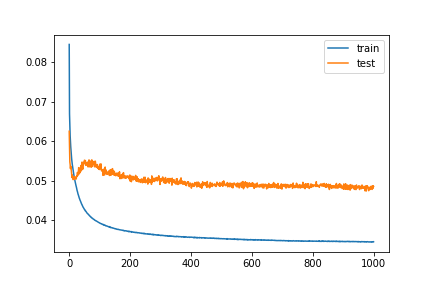
\includegraphics[scale=0.75]{conf7_1000e_15ffuture}
\begin{center}
\caption{Training and validation loss for - 15 frames input and prediction at 15-time step }
\label{fig:15-15}
\end{center}
\end{figure}

\begin{figure}[H] 
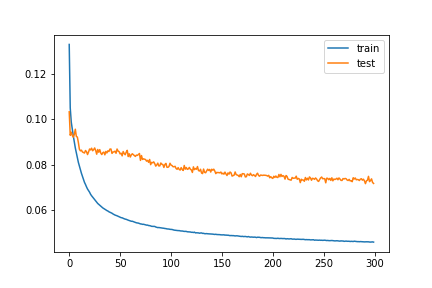
\includegraphics[scale=0.75]{conf8_300e_30ffuture}
\begin{center}
\caption{Training and validation loss for - 15 frames input and prediction at 30-time step }
\label{fig:15-30}
\end{center}
\end{figure}

\begin{figure}[H] 
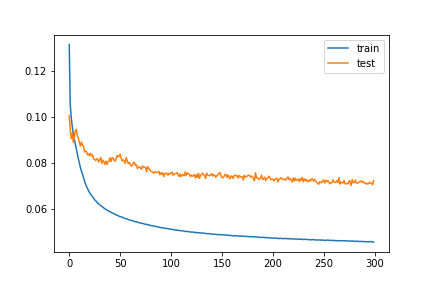
\includegraphics[scale=0.8]{conf9_300e_60ffuture}
\begin{center}
\caption{Training and validation loss for - 15 frames input and prediction at 60-time step }
\label{15-60}
\end{center}
\end{figure}

\begin{figure}[H] 
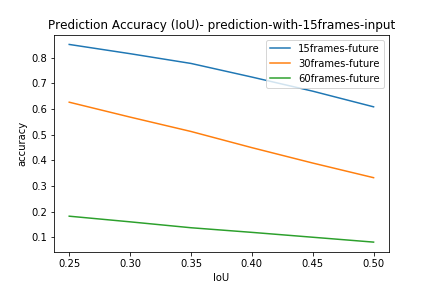
\includegraphics[scale=0.8]{prediction-with-15frames-input_IoU}
\begin{center}
\caption{Test result (IoU) for - prediction with 15 frames input}
\label{15-IoU}
\end{center}
\end{figure}

\begin{figure}[H] 
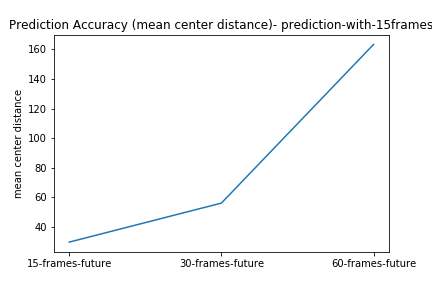
\includegraphics[scale=0.8]{prediction-with-15frames-mean_distance_accuracy}
\begin{center}
\caption{Test result (mean\textunderscore distance\textunderscore accuracy) for - prediction with 15 frames input }
\label{15-mcd}
\end{center}
\end{figure}

From the plot \ref{fig:15-15}, we can see that the validation error is least for '15 frames input and prediction at 15-time step' case. Also prediction accuracy (using IoU) from \ref{15-IoU}, for the use case, with 15 frames input and prediction at $15^{th}$ frames, it's accuracy is better than prediction at $30^{th}$ frames and $60^{th}$ frames. It is also noticeable that with an increase in the IoU for considering the prediction as accurate, the accuracy decreases linearly with the increase in IoU threshold value. When considering mean center distance as a measure of performance, the lesser the mean center distance, the better is the prediction. From the plot it is seen that, the larger the future time slice, the larger is the mean center distance.

%---------------------------------------------------------------------
\subsection{Experiment. Phase 2. Effect of different number of frames as input on prediction at 30-time step}
For Training and validation loss for - 15 frames input and prediction at 30-time step \ref{fig:15-30}

\begin{figure}[H] 
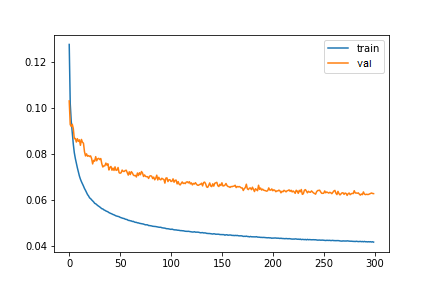
\includegraphics[scale=0.8]{conf10_300e_30ffuture}
\begin{center}
\caption{Training and validation loss for - 30 frames input and prediction at 30-time step }
\label{30-30}
\end{center}
\end{figure}

\begin{figure}[H] 
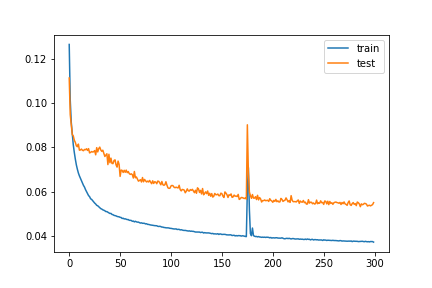
\includegraphics[scale=0.8]{conf11_300e_60_30ffuture}
\begin{center}
\caption{Training and validation loss for - 60 frames input and prediction at 30-time step }
\label{60-30}
\end{center}
\end{figure}

\begin{figure}[H] 
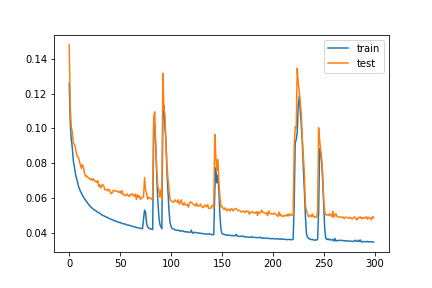
\includegraphics[scale=0.8]{conf17_300e_90_30ffuture}
\begin{center}
\caption{Training and validation loss for - 90 frames input and prediction at 30-time step }
\label{90-30}
\end{center}
\end{figure}

\begin{figure}[H] 
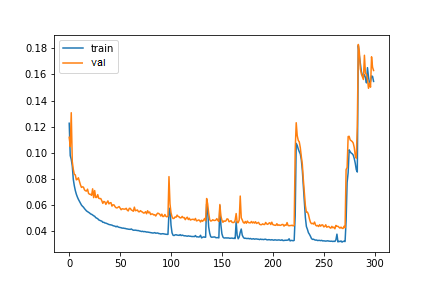
\includegraphics[scale=0.8]{conf18_300e_120_30ffuture}
\begin{center}
\caption{Training and validation loss for - 120 frames input and prediction at 30-time step }
\label{120-30}
\end{center}
\end{figure}

\begin{figure}[H] 
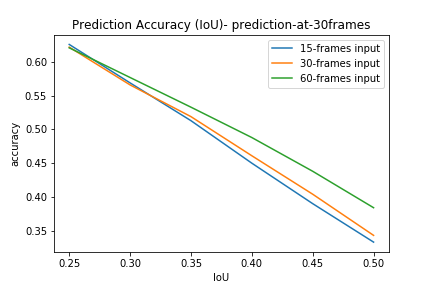
\includegraphics[scale=0.8]{prediction-at-30frames_IoU}
\begin{center}
\caption{Test result for - prediction at 30-time step }
\label{30-IoU}
\end{center}
\end{figure}

\begin{figure}[H] 
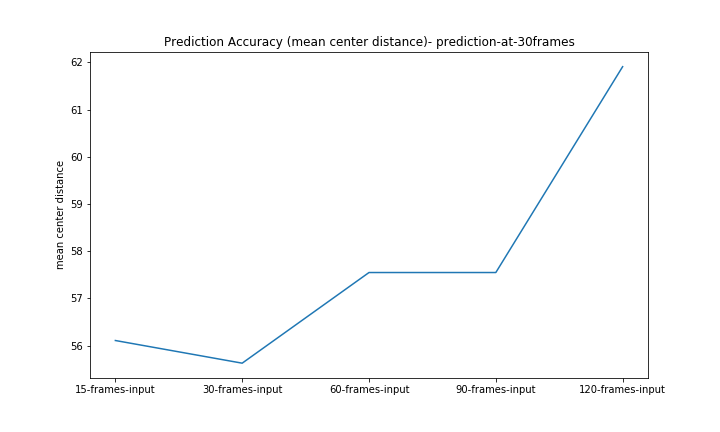
\includegraphics[scale=0.8]{prediction-at-30frames-mean_distance_accuracy}
\begin{center}
\caption{Test result (mean\textunderscore distance\textunderscore accuracy) for - prediction at 30-time step }
\label{30-mcd}
\end{center}
\end{figure}

%Test RMSE represents testing the model with frames extracted from one video from the test set.
%conf1: model with epochs = 1000, MinMaxScaler(feature\textunderscore range=(0, 1)), 
%number of sequence as observation = 3
%loss: 0.0045 - val\textunderscore loss: 0.0047 
%Test RMSE: 2.363
%Validation: Using one pedestrian bounding boxes with 205 frames.
% git commit 789d6e6

%conf2: 
%model with epochs = 200, early stopping after epoch 33
%number of sequence as observation = 15
%loss: 0.0087 - val\textunderscore loss: 0.0089
%Test RMSE: 4.749
%9c88a25

%conf3:
%model with epochs = 200, early stopping after epoch 88
%loss-0.0062 val\textunderscore loss-0.0070.h5
%model with epochs = 200
%number of sequence as observation = 30
%Test RMSE: 4.625


%conf 4  single layer, epochs 200 without early stopping
%Test data set (30 videos)
%IoU > 0.5
%avg prediction speed 0.0161
%Avg accuracy 0.39

%IoU > 0.45
%avg prediction 0.0163
%Avg accuracy 0.4416

%IoU > 0.25
%avg prediction 0.0163
%Avg accuracy 0.6603
%************************************
%conf 4 Train data set
%IoU > 0.5 0.0164 0.4483

%IoU > 0.45 0.0162 0.5106

%IoU > 0.25 0.74

%conf 5 Test data set

%val_loss improved from 0.04356 to 0.04316, saving model to conf5_epoch-281_loss-0.0296_val_loss-0.0432.h5
%Epoch 282/300
% - 999s - loss: 0.0295 - val_loss: 0.0425

%conf 5 Test data set (30 videos)
%model.add(LSTM(50, input_shape=(train_X.shape[1], train_X.shape[2]), return_sequences=True))
%model.add(Dropout(0.1))

%3 more layers

%IoU > 0.25 0.0625 0.627

%IoU > 0.45 0.0626 0.444

%IoU > 0.50 0.062 0.389

%conf 6 Test data set (30 videos)
%trained for 1000epochs
%IoU > 0.50
%0.016 0.351

%IoU > 0.45
%0.016 0.410

%IoU > 0.25
%0.016 0.636


%Conf7:
%epoch 1000
%input seq 15
%predicting 15th future frame

%They can change their walking direction in an instance,
%or start/stop walking abruptly. As a consequence, sensible prediction horizons
%are typical short (we consider < 2s in this paper).

%ls cm-pm | wc -l 185      *2  370
%ls cm-ps | wc -l 142 145  *3  335
%ls cms-pm | wc -l 245 245 *2  490
%ls cms-ps | wc -l 37 40   *12 480
%ls cs-pm| wc -l 173 175   *2  350
%ls cs-ps | wc -l 15 15    *30 450

%Train on 342135 samples, validate on 85534 samples
%Epoch 1/300
%Started at 17th sept 15:45 

%Annotations for the video can be extracted as below
%anno = imdb.\textunderscore get\textunderscore annotations(vid), this results in a dictionary which contains below keys ['height', 'ped\textunderscore annotations', 'num\textunderscore frames', 'width']

%TODO
%\newpara Weakly supervised learning!
%Sigmoid cross entropy vs  softmax
%batch normalization

%\section{LSTM with refinement}

As we can see from the above plots, the validation error is least for '60 frames input and prediction at 30-time step' case. Also prediction accuracy (using IoU) from fig \ref{30-IoU}, with 60 frames as input, the prediction accuracy is better compared to 15 frames and 30 frames as input. It is also noticeable that with an increase in the IoU for considering the prediction as accurate, the accuracy decreases linearly with an increase in IoU threshold value. When considering mean center distance as a measure of performance, the lesser the mean center distance the better is the prediction. From the plot, it is seen that for 30 frames input the prediction is slightly better than the model that takes 60 frames as input.

%---------------------------------------------------------------------
\subsection{Experiment. Phase 3. Effect of different future time stamp on prediction, with 60 frames as input}
Training and validation loss for 60 frames input and prediction at 30-time step is at \ref{60-30}

\begin{figure}[H] 
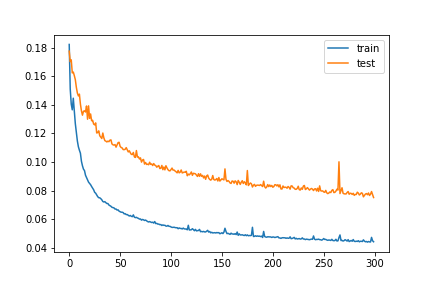
\includegraphics[scale=0.8]{conf12_300e_60_60ffuture}
\begin{center}
\caption{Training and validation loss for - 60 frames input and prediction at 60-time step }
\label{60-60}
\end{center}
\end{figure}

\begin{figure}[H] 
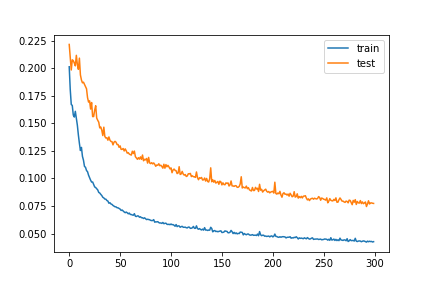
\includegraphics[scale=0.8]{conf13_300e_60_90ffuture}
\begin{center}
\caption{Training and validation loss for - 60 frames input and prediction at 90-time step }
\label{60-90}
\end{center}
\end{figure}

\begin{figure}[H] 
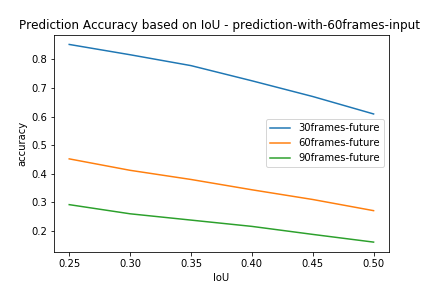
\includegraphics[scale=0.8]{prediction-with-60frames-input_IoU.png}
\begin{center}
\caption{Test result (IoU) for - prediction with 60 frames input}
\label{60-IoU}
\end{center}
\end{figure}

\begin{figure}[H] 
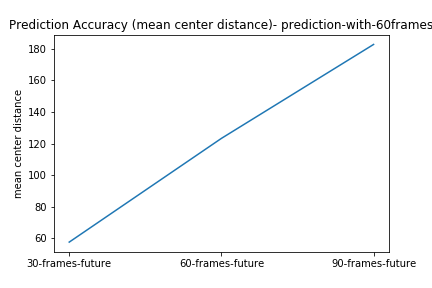
\includegraphics[scale=0.7]{prediction-with-60frames-mean_distance_accuracy}
\begin{center}
\caption{Test result (mean\textunderscore distance\textunderscore accuracy) for - prediction with 60-time step
 input }
\label{60-mcd}
\end{center}
\end{figure}

%---------------------------------------------------------------------
\subsection{Experiment. Phase 4. Effect of different units in LSTM Cell on accuracy for prediction at 90-time step with 60 frames as input}

\begin{figure}[H] 
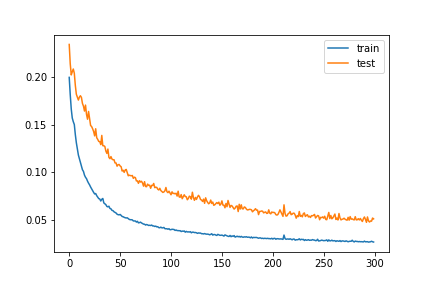
\includegraphics[scale=0.7]{conf14_300e_60_90ffuture_100unit}
\begin{center}
\caption{Training and validation loss for - 60 frames input and prediction at 90-time step using 100 units in the Cell}
\label{60-90-100unit}
\end{center}
\end{figure}

\begin{figure}[H] 
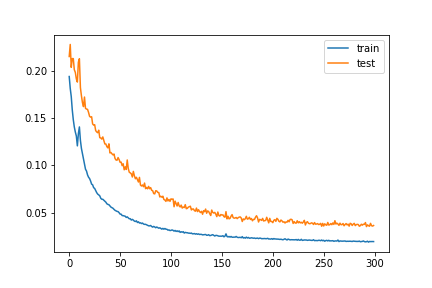
\includegraphics[scale=0.7]{conf15_300e_60_90ffuture_200unit}
\begin{center}
\caption{Training and validation loss for - 60 frames input and prediction at 90-time step using 200 units in the Cell}
\label{60-90-200unit}
\end{center}
\end{figure}

\begin{figure}[H] 
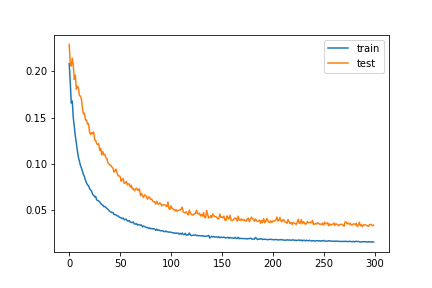
\includegraphics[scale=0.7]{conf16_300e_60_90ffuture_300unit}
\begin{center}
\caption{Training and validation loss for - 60 frames input and prediction at 90-time step using 300 units in the
 Cell}
\label{60-90-300unit}
\end{center}
\end{figure}

\begin{figure}[H] 
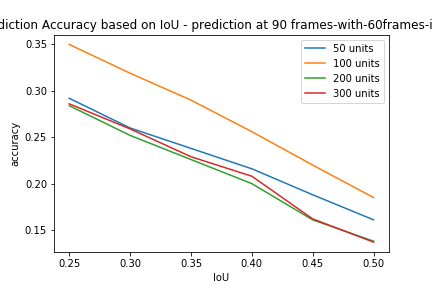
\includegraphics[scale=0.8]{prediction-at-90frames-with-60frames-input_IoU.png}
\begin{center}
\caption{Test result (IoU) for - prediction at 90 frames with 60 frame input}
\label{60-90-cell-untis-IoU}
\end{center}
\end{figure}

\begin{figure}[H] 
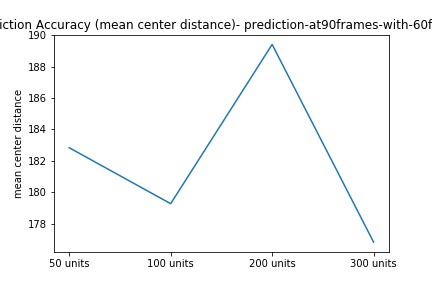
\includegraphics[scale=0.7]{prediction-at-90frames-with-60frames-mean_distance_accuracy}
\begin{center}
\caption{Test result (mean\textunderscore distance\textunderscore accuracy) for - prediction at 90 frames with 60 time step input }
\label{60-90-cell-units-mcd}
\end{center}
\end{figure}

%x = ['15_15_1000', '15_30_300', '15_60_300', '30_30_300', '60_30_300', '60_60_300', '60_90_300', '60_90_300_100', '60_90_300_200', '60_90_300_300']

%\comment{
\begin {table}[H]
\begin{center}
 \begin{tabular}{||c c c c c||} 
 \hline
conf & input frame & prediction & epoch & units\\ [1.0ex] 
\hline\hline
conf1 & 15 & 15 & 1000 & 50 \\ 
\hline
conf2 & 15 & 30 & 300 & 50 \\ 
\hline
conf3 & 15 & 60 & 300 & 50 \\ 
\hline
conf4 & 30 & 30 & 300 & 50 \\ 
\hline
conf5 & 60 & 30 & 300 & 50 \\ 
\hline
conf6 & 60 & 60 & 300 & 50 \\ 
\hline
conf7 & 60 & 90 & 300 & 50 \\ 
\hline
conf8 & 60 & 90 & 300 & 100 \\ 
\hline
conf9 & 60 & 90 & 300 & 200 \\ 
\hline
conf10 & 60 & 90 & 300 & 300 \\ 
\hline
\end{tabular}
\caption{LSTM model configuration}
\end{center}
\end{table}
%}
The above table captures various configurations are used during the experiment. \\
\textit{input frame} refers to the number of input frames the model needs for the prediction \\
\textit{prediction} refers to the frame at which the prediction is desired \\
\textit{epoch } the number of epochs the model is trained \\
\textit{units} number of units used in the LSTM cell

The below graphs depict the prediction time for the above-mentioned configurations.

\begin{figure}[H]
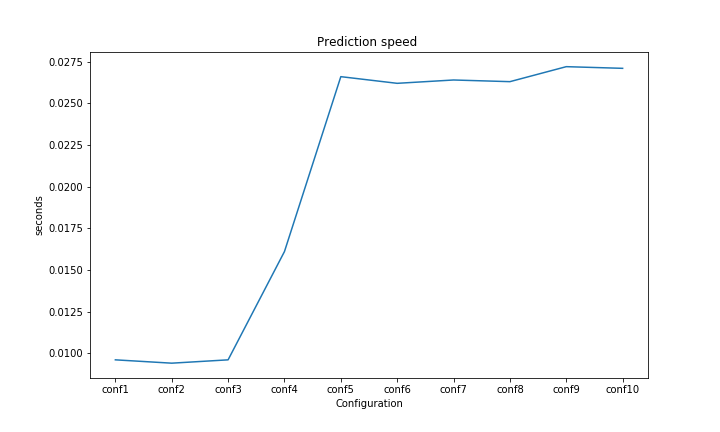
\includegraphics[scale=0.8]{time-taken-for-prediction.png}
\begin{center}
\caption{Time taken for prediction with different configuration}
\end{center}
\end{figure}

From the graph, it is seen that with an increase in the number of input time series values the prediction time increases. Changes in the number of epochs or the amount of units in the cell do not result in significant variation.

\section{SSD results}
%\subsection{Validation}
The below graphs depicts the validation error and the training error when the SSD model was trained for 10 epochs.
\begin{figure}[H]
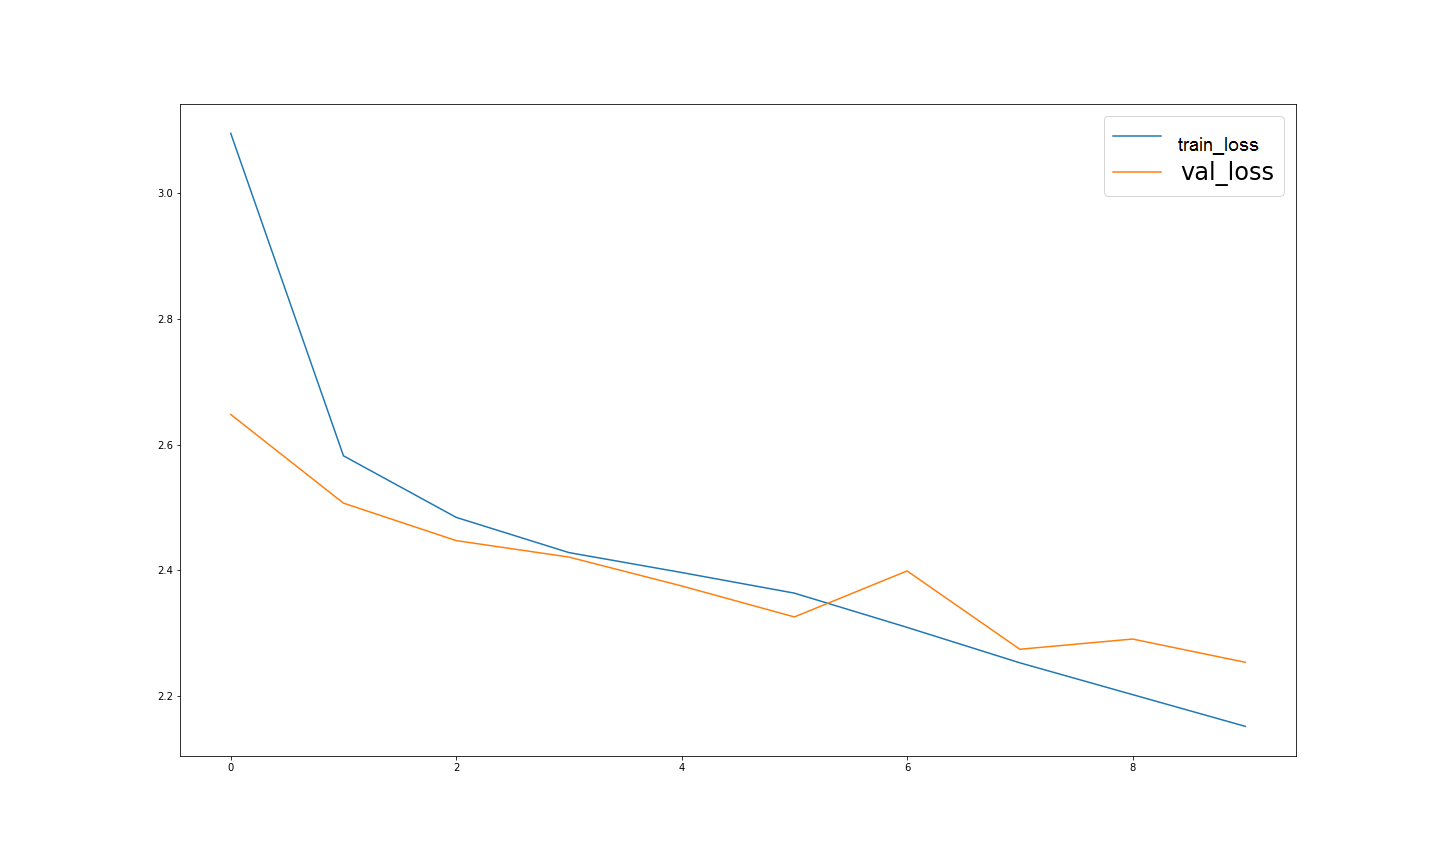
\includegraphics[scale=0.4]{conf0_loss-val_loss_0_10epochs}
\begin{center}
\caption{Training and Validation error at 10 epochs}
\end{center}
\end{figure}

As the training error has not converged after 10 epochs, it was decided to train for another 10 epoch and the graph as shown below. After training for 10 more epochs the training error gradually reduces. The validation error that revolves around training error is shown in the below graph. As the training of a single epoch takes significant time, the statistics were taken with small epochs.

\begin{figure}[H]
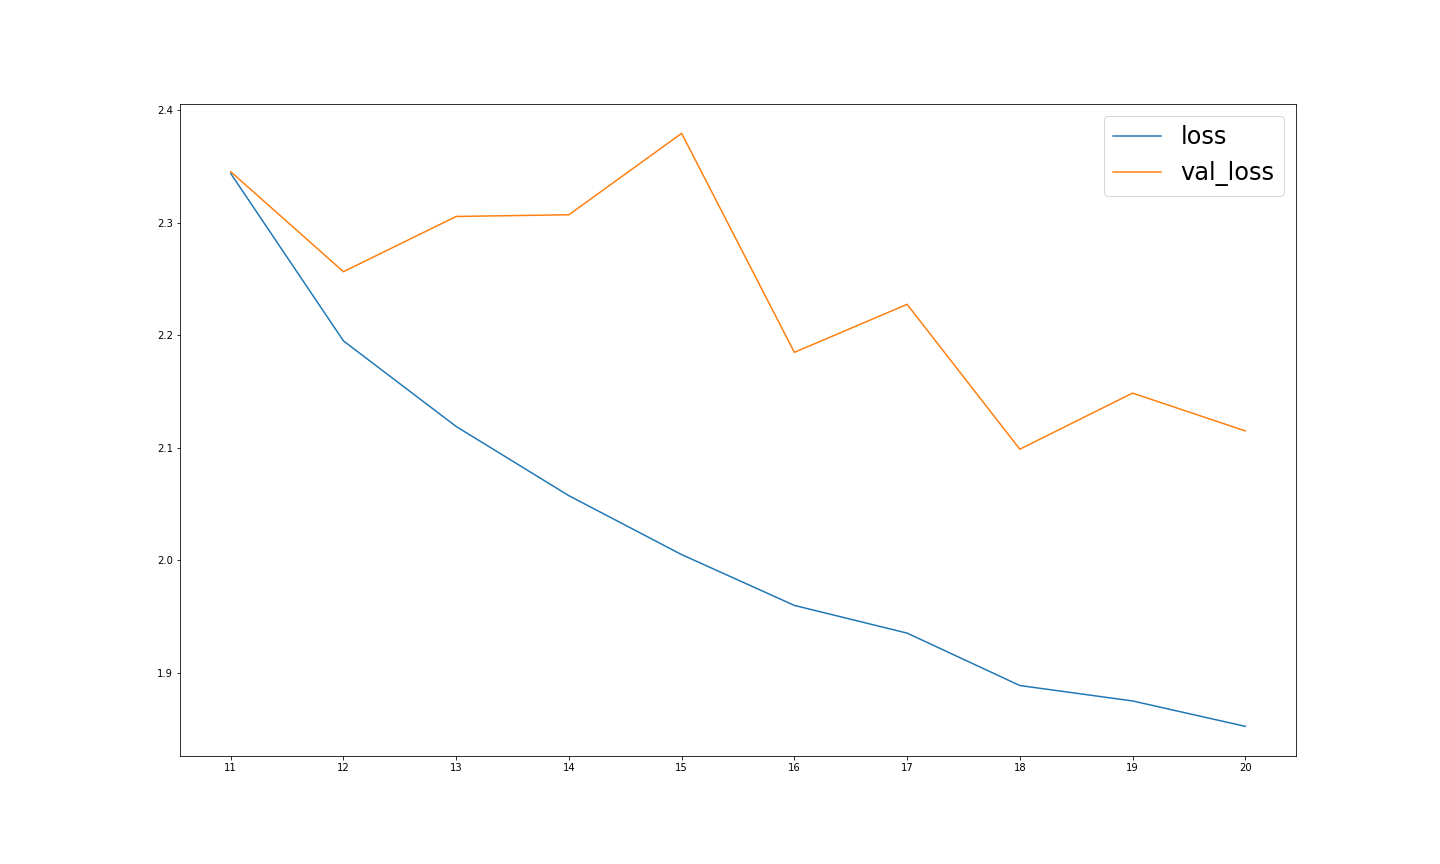
\includegraphics[scale=0.4]{conf0_loss-val_loss_10_20epochs}
\begin{center}
\caption{Training and Validation error at 20 epochs}
\end{center}
\end{figure}

\newpara
Looking at the graph which depicts training loss and validation loss has drawn with several epochs, we could see training error gradually reduces with an increase in the number of epochs, simultaneously we see validation loss also exhibiting the same pattern and slowly decreasing with the number of epochs. This trend of decrease in validation error with an increase in training is a good indication of learning. The model could have trained for some more epochs until it converges, however, due to long training time, it was not possible to do so, instead training with different configuration was done to see the behavior with other configuration.

%\subsection{Testing} 
For the testing of the generated model below steps were followed to prepare the test data and conduct the experiment.
\begin{enumerate}
	\item video set 06 - 10 was selected as test data and bounding box, label is extracted into labels\textunderscore test\textunderscore full.csv which contains total 154436 records
	\item Rows with occluded and other classes except person were removed and the remaining number of records were 73218, which consists of 42910 unique images 
	\item records with less than 50 pixels for height or 5 pixels for width were discarded and data set left with 29620 records
	\item From the above data, 1000 records were randomly chosen for test purpose which consists of 902 unique images
\end{enumerate}

\newpara
While using SSD7, it was observed that the algorithm is very sensitive to the list of aspect ratios for the anchor boxes. To begin with, the values for aspect\textunderscore ratios = $[0.5, 1.0, 2.0]$ were used and that lead to a very poor results in the evaluation phase. Subsequently, the model was trained with several different configuration and results are noted as below.

for aspect\textunderscore ratios = $[0.1, 0.2, 0.33, 0.413, 0.418, 0.5, 0.6, 0.7, 0.8, 1.0]$
\begin{table}[H]
\begin{center}
 \begin{tabular}{||c c c||} 
 \hline
 No. epoch & mAP & fps\\ [0.8ex] 
 \hline\hline
 10 & 0.661 & 10.22\\ 
 \hline
 20  & 0.635 & 9.73 \\
\hline
\end{tabular}
\caption{Average Precision and fps with the number of epochs}
\end{center}
\end{table}
From the above result, it can be observed that training the data for more epochs is actually not resulting in a better model as both mAP and fps are lowered for the model trained with 20 epochs, this could be a sign of \textit{over-fitting.}

%conf1
%0.2, 0.33, 0.413, 0.418, 0.5, 0.6, 0.7, 0.8, 1.0
%0.4376
%fps 73.14

%conf 2
%epoch 5
%0.1, 0.2, 0.33, 0.413, 0.418, 0.5, 0.6, 0.7, 0.8
%fps: 75.58 
%mAP:0.471

%conf 3 
%0.1, 0.2, 0.33, 0.413, 0.418, 0.5, 0.6, 0.7, 0.8, 1.0

With the increase in the number of values in the list of aspect ratio, the number of predictor boxes increases. An increase in the number of predictor boxes increases both training time as well as prediction time.
